%%%%%latex preamble%%%%%
\documentclass[titlepage]{article}\usepackage[]{graphicx}\usepackage[]{color}
%% maxwidth is the original width if it is less than linewidth
%% otherwise use linewidth (to make sure the graphics do not exceed the margin)
\makeatletter
\def\maxwidth{ %
  \ifdim\Gin@nat@width>\linewidth
  \linewidth
  \else
  \Gin@nat@width
  \fi
}
\makeatother


\usepackage{listings}
\definecolor{mygreen}{rgb}{0,0.6,0}
\definecolor{mygray}{rgb}{0.5,0.5,0.5}
\definecolor{mymauve}{rgb}{0.58,0,0.82}
\lstset{ %
  backgroundcolor=\color{white},   % choose the background color; you must add \usepackage{color} or \usepackage{xcolor}
  basicstyle=\footnotesize,        % the size of the fonts that are used for the code
  breakatwhitespace=false,         % sets if automatic breaks should only happen at whitespace
  breaklines=true,                 % sets automatic line breaking
  captionpos=b,                    % sets the caption-position to bottom
  commentstyle=\color{mygreen},    % comment style
  deletekeywords={...},            % if you want to delete keywords from the given language
  escapeinside={\%*}{*)},          % if you want to add LaTeX within your code
  extendedchars=true,              % lets you use non-ASCII characters; for 8-bits encodings only, does not work with UTF-8
  frame=single,                    % adds a frame around the code
  keepspaces=true,                 % keeps spaces in text, useful for keeping indentation of code (possibly needs columns=flexible)
  keywordstyle=\color{blue},       % keyword style
  language=Python,                 % the language of the code
  morekeywords={*,...},            % if you want to add more keywords to the set
  numbers=left,                    % where to put the line-numbers; possible values are (none, left, right)
  numbersep=5pt,                   % how far the line-numbers are from the code
  numberstyle=\tiny\color{mygray}, % the style that is used for the line-numbers
  rulecolor=\color{black},         % if not set, the frame-color may be changed on line-breaks within not-black text (e.g. comments (green here))
  showspaces=false,                % show spaces everywhere adding particular underscores; it overrides 'showstringspaces'
  showstringspaces=false,          % underline spaces within strings only
  showtabs=false,                  % show tabs within strings adding particular underscores
  stepnumber=2,                    % the step between two line-numbers. If it's 1, each line will be numbered
  stringstyle=\color{mymauve},     % string literal style
  tabsize=2,                       % sets default tabsize to 2 spaces
  title=\lstname                   % show the filename of files included with \lstinputlisting; also try caption instead of title
}
\usepackage{alltt}
\usepackage[sc]{mathpazo}
\usepackage{amsmath, amsthm, amssymb}
\usepackage{graphicx}
\usepackage[T1]{fontenc}
\usepackage{geometry}
\geometry{verbose,tmargin=2.5cm,bmargin=2.5cm,lmargin=1.5cm,rmargin=1.5cm}
\setcounter{secnumdepth}{2}
\setcounter{tocdepth}{2}
\usepackage{url}
\usepackage[unicode=true,pdfusetitle,
  bookmarks=true,bookmarksnumbered=true,bookmarksopen=true,bookmarksopenlevel=2,
breaklinks=false,pdfborder={0 0 1},backref=false,colorlinks=false]
{hyperref}
\hypersetup{pdfstartview={XYZ null null 1}}
\usepackage{float}
\usepackage{bm}
\usepackage{tikz}
 %changes default sectioning commands -> 1,a, etc.
%\usepackage{breakurl}
\renewcommand{\thesubsection}{(\alph{subsection})}
\renewcommand{\thesubsubsection}{\roman{subsection}.}
\usepackage{lastpage}
\usepackage{fancyhdr}
\pagestyle{fancy}
\usetikzlibrary{automata,positioning}
%%% Header and Footer %%% 
\lhead{}
\chead{\leftmark}
\rhead{}
\lfoot{Ahmad Darki; Theory of Computation}
\cfoot{Homework 2}
\rfoot{Page \thepage\ of \pageref{LastPage}}
\IfFileExists{upquote.sty}{\usepackage{upquote}}{}

\begin{document}

\title{More Fun With Automata \\ Homework 2, CS500, Fall 2014}
\author{Ahmad Darki, \\ group 11}
\maketitle


%%%%%%%%%%%%%%%%%%%%%%%%%%%%%%%%%%%%%%%%%%%%%%%%
\section*{Ex 7}
\begin{quote}
  \textbf{Show that if $L$ is regular then $L^∗$ is regular. Why does it not suffice
  to use the fact that the regular languages are closed under concatenation and
  union?}
\end{quote}
\subsubsection*{Answer:}

Since $L$ is a regular language over alphabet $A$,with states of $S$, accepting states of $S^{yes}$, start state of $S^0$ and the transition function of $\delta$ then it can be recognized by an $DFA$:

\[ 
  M = (S, A, S^0, S^{yes}, \delta)
\]

Also $L^*$, also know as \textit{Kleene star} is defined as follow:

\[
  L^* = \epsilon \cup L \cup LL \cup LLL \cup ... = \{w_1w_2...w_t | t \geq 0, w_i \in L for all 1 \leq i \leq t\}
\]

In $L^*$ the conversion changes to a unions of concatenation of language $L$. According to $L$ we know that this $DFA$ has accepting states of $S^{yes}$ where with an $\epsilon$ transition we can connect the accepting state to the start state again. This will create the concatenation of multiple of $L$.

As it is mentioned within the notes the union of regular languages is a regular language as well, and more over the concatenation of regular languages is also regular. This shows that the $L^*$ which is a combination of both union and concatenation is also will be regular language. Also it is known that an empty language denoted as $\epsilon$ is also a regular language.

\vspace{1cm}


%%%%%%%%%%%%%%%%%%%%%%%%%%%%%%%%%%%%%%%%%%%%%%%%

\section*{Ex 8}
\begin{quote}
  \textbf{Given a string $w$ , let $w^R$ denote $w$ written in reverse.
    Given a language $L$, let $L^R = \{w^R | w \in L \}$. Prove that $L$ is regular if and
    only if $L^R$ is regular. Why is this harder to prove with DFAs?}
\end{quote}
\subsubsection{Prove $L$ is regular if $L^R$ is regular}
Since $L$ is regular, there is a $DFA$ that describes this language:

\[ 
  M = (S, A, S^0, S^{yes}, \delta)
\]

Having this we assume an $NFA$ for $L^R$ that is described as followed:

\[ 
  M^{\prime} = (S \cup \{S^{0\prime}\}, A, S^{0\prime}, S^{yes}, \delta^{\prime})
\]

And for this $NFA$ we assume have the following transitions:

\[ 
  \delta^{\prime}(S^{0\prime}, a) = \emptyset ~~~~~~ a is a string from A~~~~~~ (I)
\]

\[ 
  \delta^{\prime}(S^{0\prime}, \epsilon) = S^{yes}~~~~~~ (II)
\]

\[ 
  \delta^{\prime}(s, a) = \{s^{\prime} | \delta(s^{\prime}, a) = s\} 	~~~~~~	s \in S and a is a string from A ~~~~~~ (III)
\]

We know that $w \in L(M)$ which can be cracked into $w_1 w_2 w_3 ... w_n$ and the transition of each part of this string is being done within these states $s_0,s_1,s_2,s_3,...,s_n$ where $s_0=S^0$ which indicates the starting state, also $s_n \in S^{yes}$ and for each transition we have $\delta(s_{i-1}, w_i) = s_i$. For $w^R$ we have $\epsilon w_n w_{n-1} ... w_2 w_1 $ with transitions of $S^{0\prime}, s_n, s_{n-1}, ..., s_1$ which implies that $S^{0\prime}$ is the initial state and $s_1$ is both accepting state for $w^R$ and is the $S^0$ for $w$. Having said this we only need to prove that each transitions over $M^{\prime}$ is valid. Given the transition $II$ on $\delta^{\prime}(S^{0\prime}, \epsilon) = S^{yes}$ we know that $r_n$ satisfies the transition, which can also be seen as $r_n \in \delta^{\prime}(S^{0\prime}, \epsilon) \Longrightarrow r_n \in S^{yes}$. For the rest of the string with respect to $III$ transition, it follows the $w \in L(M)$ when we assume that $r_{i-1} \in \delta^{\prime}(s_i, w_i)$.
This proves that $L(M^\prime)$ is regular since it can be accepted by an $NFA$
\subsubsection{Prove $L^R$ is regular if $L$ is regular}
This prove is like above as we have $w \in L(M^{\prime})$ which is broken into $w_1 w_2 w_3 ... w_n$ and as well the transition of the states are $s_0,s_1,s_2,s_3,...,s_n$ such that $s_0$ is the initial state and $s_n \in S^{yes}$ indicating the accepting state and furthermore the transition functions are $s_{i+1} \in \delta^{\prime}(s_i, w_{i+1}$. Also given the transitions of $I$, $II$, and $III$ as a result $w_1 = \epsilon$ and $s_r \in S^{yes}$ and all the states are $\in S$.
Now we assume $w^R$ is $w_n w_{n-1}...w_2$ with the successive states of $s_n,s_{n-1},...,s_1$ where $s_n$ is the starting state and $r_1$ is the accepting state meaning $s_1 \in S^yes$. So the remaining of this proof is to only show that the transition is valid to this $DFA$ meaning: $s_{i-1} = \delta(s_i, w_i)$. Which can be proven by conducting $s_i \in \delta^{\prime}(s_{i-1}, w_i)$ and $s_i \in \{s|\delta(s, w_i) = r_{i-1}\}$.
\vspace{1cm}



%%%%%%%%%%%%%%%%%%%%%%%%%%%%%%%%%%%%%%%%%%%%%%%%

\section*{Ex 11}
\begin{quote}
    \textbf{Given finite words $u$ and $v$, say that a word $w$ is an interweave of $u$ and $v$ if I can get $w$ by peeling off symbols of $u$ and $v$, taking the next symbol of $u$ or the next symbol of $v$ at each step, until both are empty. (Note that w must have length $|w| = |u| + |v|$.) For instance, if $u = cat$ and $v = tapir$, then one interleave of $u$ and $v$ is $w = ctaapitr$. Note that, in this case, we don't know which $a$ in $w$ came from $u$ and which came from $v$. Now given two languages $L_{1}$ and $L_{2}$, let $L_{1} \wr L_{2}$ be the set of all interweaves $w$ of $u$ and $v$, for all $u \in L_{1}$ and $v \in L_{2}$. Prove that if $L_{1}$ and $L_{2}$ are regular, then so is $L_{1} \wr L_{2}$.}
  
\end{quote}
\subsubsection*{Answer:}
We assume $L_1 \wr L_2$ is a language that can be described by the following:

\[ 
  M_{L_inter} = (S, A, S^0, S^{yes}, \delta)
\]

and $L_1$ as:

\[ 
  M_{L_1} = (S_{L_1}, A, S_{L_1}^0, S_{L_1}^{yes}, \delta_{L_1})
\]

and $L_2$ as:

\[ 
  M_{L_2} = (S_{L_2}, A, S_{L_2}^0, S_{L_2}^{yes}, \delta_{L_2})
\]

Let's take  $L_cartesian12$ to be the \textit{Cartesian product} of the two languages $L_1$ to $L_2$. Where the language will be as: 

\[ 
  M_{L_cartesian12} = (S_{L_1} \times S_{L_2}, A, (S_{L_1}^0, S_{L_2}^0), (S_{L_1}^{yes} \cup S_{L_2}^{yes}), \delta_{L_1} \times \delta_{L_2} )
\]

and also the $L_cartesian21$ will be the \textit{Cartesian product} of $L_2$ to $L_1$":

\[ 
  M_{L_cartesian21} = (S_{L_2} \times S_{L_1}, A, (S_{L_2}^0, S_{L_1}^0), (S_{L_1}^{yes} \cup S_{L_2}^{yes}), \delta_{L_2} \times \delta_{L_1} )
\]

as we know that \textit{Cartesian product} of two regular language is also a regular language. Also the union of two regular languages will be a regular language itself. The idea is to take the interweave as a result of union over the two \textit{Cartesian product}.

\textbf{I can not prove what I'm trying to say here....!!!}
\vspace{1cm}


%%%%%%%%%%%%%%%%%%%%%%%%%%%%%%%%%%%%%%%%%%%%%%%%

\section*{Ex 10}
\begin{quote}
  \textbf{
  A parity finite-state automaton, or $PFA$ for short, is like an $NFA$ except that it accepts a string $w$ if and only if the number of accepting paths induced by reading $w$ is odd. Show how to simulate a $PFA$ with a $DFA$, and thus prove that a language is recognized by a $PFA$ if and only if it is regular. Hint: this is a little trickier than our
  previous simulations, but the number of states of the $DFA$ is the same.}
\end{quote}

\subsubsection*{Answer:}
Assume an $NFA$ being regular:

\[ 
  M_2 = (S_2, A, S^0_2, S^{yes}_2, \delta_2)
\]
From this $NFA$ we will have a $DFA$ as:

\[ 
  M = (S, A, S^0, S^{yes}, \delta)
\]

Where $S = 2^{S_2}$, $S^{yes} = {S^{yes}_2}$, $\delta(T, a) = \cup_{t\in T} \delta_2(t, a)$, and $S^{yes} = \{T\cap S^{yes}_2\}$ in which this $DFA$ is regular as well. For this problem we need to prove that for an odd number of  $\delta_2(S^0_2, w) = s^{yes}_2 \in S^{yes}_2$ we will be able to make another $DFA$. From this we know that there will be an odd number of transitions of $\delta_2(S^0_2, w)$ which means $|w|$ is an odd number as in $w=w_1w_2...w_(2n+1)$.
\vspace{1cm}



%%%%%%%%%%%%%%%%%%%%%%%%%%%%%%%%%%%%%%%%%%%%%%%%
\section*{Ex 13}
\begin{quote}
  \textbf{Show that if $u \sim_L v$ , then $ua \sim_L va$ for any $a \in A$.}
\end{quote}

\subsubsection*{Answer:}
Having known that for a given language $L \subseteq A^* $ we say that a pair of $u, v \in A^*$ are equivalent with respect to L, denoted as $u \sim_L v$ if for all $w \in A^*$ we have:

\[
	uw \in L \text{ iff } vw \in L.
\]
we then split up $w$ into $az$ where $a \in A$ and $z \in L$. We know the $M$, the language, will accept the both $u$ and $v$ in sense that the final state of the both strings will be the same, and the $w$ will take the state into the accepting state. So the idea of splitting $w$ into $az$ will take the state to first: state of receiving $a$ and then the rest of the state of with the input string of $z$ which will go to the accepting state since $z \in L$.
\vspace{1cm}



%%%%%%%%%%%%%%%%%%%%%%%%%%%%%%%%%%%%%%%%%%%%%%%%
\section*{Ex 14}
\begin{quote}
  \textbf{Describe the equivalence classes of the three languages from Exercise
  2. Use them to give the minimal DFA for each language, or prove that the DFA
  you designed before is minimal.}
\end{quote}
\subsubsection{Exercise 2.2: The set of strings in $\{a, b, c\}^*$ where there is no $c$ anywhere to the left of an $a$.}
As it has been proven that the following DFA is a minimal, with respect to the number of states the \textit{equivalence class} are 3 as followed:

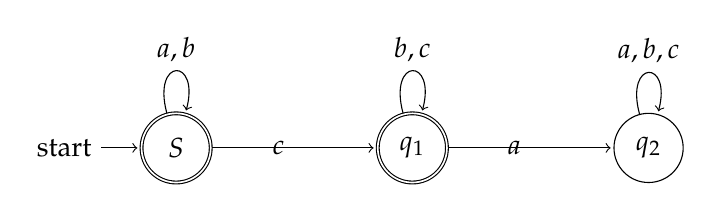
\begin{tikzpicture}[shorten >=1pt,auto,node distance=3 cm, scale = 1, transform shape]


\node[initial,state,accepting] (S)                                    {$S$};
\node[state,accepting]         (B) [right of=S]                       {$q_1$};
\node[state]                   (C) [right of=B]					      {$q_2$};

\path[->]
      (S) edge [loop above]      node [align=center]  {$ a, b $} (S)
      (S) edge [left]       node [align=center]  {$ c $} (B)
      (B) edge [loop above]      node [align=center]  {$ b, c $} (B)
      (B) edge [left] node [align=center]  {$ a $} (C)
      (C) edge [loop above] node [align=center]  {$ a, b, c $} (C);
\end{tikzpicture}

\begin{enumerate}
  \item $[\epsilon] = [a] = [ab] = [aba]$, The set of strings in $w$ without any $c$.
  \item $[c] = [cb] = [cbc]$, The set of strings in $w$ starting with $c$.
  \item $[c] = [cb] = [cbc] = [cbcb] = [cbcba]$, The set of strings in $w$ where there is $c$ to the left of $a$
\end{enumerate}

\vspace{1cm}




%%%%%%%%%%%%%%%%%%%%%%%%%%%%%%%%%%%%%%%%%%%%%%%%
\section*{Ex 20}
\begin{quote}
  \textbf{Consider the language}
  \[ L_{a=b,c=d } = \{ w \in \{a,b, c ,d \}^* \, | \#_a (w) = \#_b (w) \text{ and }
    \#_c (w) = \#_d (w )
  \]
  
\textbf{What are its equivalence classes? What does its minimal infinite-state machine
look like?}
\end{quote}

\subsubsection{Answer:}

\begin{tikzpicture}[shorten >=1pt,auto,node distance=2 cm, scale = 1, transform shape]


\node[state,accepting] (S)                                    {$0$};
\node[state]         (A) [right of=S]                       {$1$};\\
\node[state]         (B) [right of=A]                       {$2$};

\node[state]         (C) [left of=S]                        {$-1$};
\node[state]         (D) [left of=C]					    {$-2$};

\node[state]         (E) [above of=S]                       {$-1$};
\node[state]         (F) [above of=E]                       {$-2$};

\node[state]         (G) [below of=S]                       {$1$};
\node[state]         (H) [below of=G]                       {$2$};
\path[->]
      (S) edge [left]      node   {$ b $} (C)
      (S) edge [bend right]     node  {$ a $} (A)
      
      (A) edge [left]      node {$ b $} (S)
      (B) edge [left]      node {$ b $} (A)
      (C) edge [left]      node {$ b $} (D)
      
      (D) edge [bend right]      node {$ a $} (C)
      (C) edge [bend right]      node {$ a $} (S)
      (A) edge [bend right]      node {$ a $} (B)
      
      (S) edge       node   {$ c $} (E)
      (S) edge       node {$ d $} (G)
      
      (E) edge      node {$ c $} (F)
      (H) edge       node  {$ c $} (G)
      (G) edge      node {$ c $} (S)
      
      (F) edge       node {$ d $} (E)
      (E) edge       node {$ d $} (S)
      (G) edge       node {$ d $} (H);
\end{tikzpicture}


\textbf{I can not fix this tikz...}


In this problem, the number of elements is taken into consideration. This can not be done using any type of Automata since the number of elements had been taken into account which requires the machine to have infinite states as shown above. As well this language can not be described using regular expressions.
\vspace{1cm}




\end{document}
